\documentclass[12pt]{article}
\usepackage{amssymb}
\usepackage{amsfonts}
\usepackage{amsmath} 
\usepackage{bm}
\usepackage{graphicx}
\usepackage{cancel}
\usepackage{enumitem}
\usepackage{fancyhdr}
\usepackage{fancyvrb}
\usepackage[paperwidth=8.5in,paperheight=11in,margin=1in]{geometry}

\pagestyle{fancy}
\lhead{Peter Williams}
\chead{Carroll and Ostlie Notes}
\rhead{\today}

\begin{document}
\section{The Celestial Sphere}

\section{Celestial Mechanics}

\section{The Continuous Spectrum of Light}
\begin{itemize}
\item Stellar parallax: 
\begin{equation}
d = \frac{1\text{ AU}}{\tan p} \approx \frac{1}{p}\text{ AU}
\end{equation}
\begin{itemize}
\item parsec: distance when parallax angle is 1 arcsecond.
\item Hipparcos (ESA): accuracies approaching 0.001$^{\prime\prime}$
\item Gaia: accuracies approaching 4 microarcsec
\end{itemize}
\item apparent magnitude:
\begin{itemize}
\item difference of 5 magnitudes = factor of 100 difference in brightness $\Longrightarrow$ $100^{1/5} = 2.512$
\item Solar constant: 1.4 kW m$^{-2}$
\item
\begin{equation}
\frac{F_2}{F_1} = 100^{(m_1-m_2)/5} \Longrightarrow m_1 - m_2 = -2.5\log_{10}\left(\frac{F_1}{F_2}\right)
\end{equation}
\end{itemize}
\item absolute magnitude:
\begin{itemize}
\item apparent magnitude at 10 kpc
\item distance modulus
\begin{align*}
100^{(m - M)/5} = \frac{F_{10}}{F} = \left(\frac{d}{10\text{ pc}}\right)^2 &\Longrightarrow d = 10^{(m - M + 5)/5}\text{ pc} \\
&\Longrightarrow m - M = 5\log_{10}(d) - 5 = 5\log_{10}\left(\frac{d}{10\text{ pc}}\right)
\end{align*}
\end{itemize}
\item Double slit experiment:
\begin{itemize}
\item spacing $d$ between slits, distance $L$ to screen. At angle $\theta$, extra path length of $d\sin\theta$ for far slit $\Longrightarrow$ bright if $d\sin\theta = n\lambda$, dark if $d\sin\theta = (n - \frac{1}{2})\lambda$.
\end{itemize}
\item Poynting vector:
\begin{equation}
\bm{S} = \frac{1}{\mu_0}\bm{E}\times\bm{B}\text{ (SI)} = \frac{c}{4\pi}\bm{E}\times\bm{B}\text{ (cgs)}
\end{equation}
\begin{itemize}
\item radiation pressure:
\begin{align*}
F_{rad} &= \frac{\langle S\rangle A}{c}\cos\theta~~~~~~~~~\text{(absorption)}\\
F_{rad} &= \frac{2\langle S\rangle A}{c}\cos^2\theta~~~~~~\text{(reflection)}
\end{align*}
\end{itemize}
\item Blackbodies:
\begin{itemize}
\item Wien's displacement law:
\begin{equation}
\lambda_\text{max} T = 0.002897755\text{ m K}
\end{equation}
\item Stefan-Boltzmann equation:
\begin{equation}
L = A\sigma T^4,~~~~\sigma = 5.67\times 10^{-8}\text{ W m}^{-2}\text{K}^{-4}.
\end{equation}
\item Rayleigh-Jeans law: works for $\lambda$ large. Take oven with distance $L$ between walls, then can have standing waves with wavelength $\lambda = 2L/1, 2L/2, 2L/3, 2L/4, 2L/5, \dots,$ each wavelength with energy $kT$. Then (DERIVATION --- LEARN)
\begin{equation}
B_\lambda(T)\approx\frac{2ckT}{\lambda^4}
\end{equation}
\item Wien's approximation: works for $\lambda$ small. (DERIVATION --- LEARN)
\begin{equation}
B_\lambda(T) \approx a \lambda^{-5} e^{-b/\lambda T}
\end{equation}
\item Planck:
\begin{equation}
B_\lambda(T) = \frac{a/\lambda^5}{e^{b/kT} - 1}
\end{equation}
Assume energy must be quantized: $nh\nu$. (DERIVATION --- LEARN)
\begin{equation}
B_\lambda(T) = \frac{2hc^2/\lambda^5}{e^{hc/\lambda k T} - 1}
\end{equation}
$\lambda = c/\nu$, so $d\lambda = c/\nu^2 d\nu$:
\begin{equation}
B_\nu(T) = \frac{2 h \nu^3/c^2}{e^{h\nu/k T} - 1}
\end{equation}
\end{itemize}
\item Color index
\begin{align*}
U - B &= M_U - M_B \\
B - V &= M_B - M_V
\end{align*}
\begin{itemize}
\item Bolometric correction:
\begin{equation}
BC = m_\text{bol} - V = M_\text{bol} - M_V
\end{equation}
\item Sensitivity function $S(\lambda)$
\begin{equation}
U = -2.5\log_{10}\left(\int_0^\infty F_\lambda S_U d\lambda\right)+C_U
\end{equation}
$C_U$ chosen such that Vega has magnitude zero in each filter.
\begin{equation}
U - B = -2.5\log_{10}\left(\frac{\int F_\lambda S_U d\lambda}{\int F_\lambda S_B d\lambda}\right)+C_{U-B},~~C_{U-B} \equiv C_U - C_B
\end{equation}
\item *** Color index does not depend on distance, so it is a measure solely of the temperature of a model blackbody star
\end{itemize}
\end{itemize}

\section{The Theory of Special Relativity}
\begin{itemize}
\item Galilean transformations:
\begin{eqnarray}
x^\prime &= &x - ut \\
y^\prime &= &y \\
z^\prime &= &z \\
t^\prime &= &t
\end{eqnarray}
\begin{equation}
\bf{v}^\prime = \bf{v} - \bf{u},~~\bf{a}^\prime = \bf{a}
\end{equation}

\item Michelson-Morley Experiment - no ether

\item Lorentz transformations:
\begin{eqnarray}
x^\prime &= &\frac{x - ut}{\sqrt{1 - u^2/c^2}} \\
y^\prime &= &y \\
z^\prime &= &z \\
t^\prime &= &\frac{t - ux/c^2}{\sqrt{1 - u^2/c^2}}
\end{eqnarray}
\begin{equation}
\gamma \equiv \frac{1}{\sqrt{1-u^2/c^2}}
\end{equation}
\begin{itemize}
\item Time dilation:
\begin{equation}
\Delta t_\text{moving} = \frac{\Delta t_\text{rest}}{\sqrt{1-u^2/c^2}}
\end{equation}
\item Length contraction:
\begin{equation}
L_\text{moving} = L_\text{rest}\sqrt{1-u^2/c^2}
\end{equation}
\item Relativistic Doppler shift:
\begin{equation}
\nu_\text{obs} = \frac{\nu_\text{rest}\sqrt{1-u^2/c^2}}{1+(u/c)\cos\theta} = \frac{\nu_\text{rest}\sqrt{1-u^2/c^2}}{1+v_r/c}
\end{equation}
\begin{equation}
\Longrightarrow \nu_\text{obs} = \nu_\text{rest}\sqrt{\frac{1 - v_r/c}{1+v_r/c}} ~~~~~~~(\text{radial motion})
\end{equation}
***Note that there is still a transverse Doppler shift
\end{itemize}
\item Cosmological redshift:
\begin{equation}
z\equiv \frac{\lambda_\text{obs} - \lambda_\text{rest}}{\lambda_\text{rest}} = \frac{\Delta \lambda}{\lambda_\text{rest}}
\end{equation}
\begin{itemize}
\item For $u/c << 1$, $z\approx v_r/c$.
\end{itemize}
\item Velocity transformations:
\begin{eqnarray}
v_x^\prime &= &\frac{v_x - u}{1 - uv_x/c^2} \\
v_y^\prime &= &\frac{v_y\sqrt{1 - u^2/c^2}}{1 - uv_x/c^2} \\
v_z^\prime &= &\frac{v_z\sqrt{1 - u^2/c^2}}{1 - uv_x/c^2}
\end{eqnarray}
\item Relativistic beaming: Consider a light source moving in the positive $x$-direction with relativistic speed $u$. Consider light ray traveling in the $y$ direction (at speed $c$) in the light source's rest frame. Then
\begin{equation}
v_x = \frac{v_x^\prime + u}{1 - uv_x^\prime/c^2} = u
\end{equation}
\begin{equation}
v_y = \frac{v_y^\prime\sqrt{1-u^2/c^2}}{1+uv_x^\prime/c^2} = c\sqrt{1 - u^2/c^2}
\end{equation}
\begin{equation}
v_z = \frac{v_z^\prime\sqrt{1 - u^2/c^2}}{1 + u v_x^\prime/c^2} = 0
\end{equation}
\begin{equation}
\Longrightarrow \sin\theta = v_y/c = \gamma^{-1}
\end{equation}

\item Relativistic momentum:
\begin{equation}
{\bf p} = \frac{m{\bf v}}{\sqrt{1 - v^2/c^2}} = \gamma m {\bf v}
\end{equation}

\item Relativstic kinetic energy:
\begin{equation}
K = \int_{x_i}^{x_f} F dx = \int_{x_i}^{x_f}\frac{dp}{dt}dx =  \int_{p_i}^{p_f}\frac{dx}{dt}{dp} = \int_{p_i}^{p_f} v dp
\end{equation}
Using $p_i = 0$ and integrating by parts, 
\begin{align}
K &= p_fv_f - \int_0^{v_f} p dv \\
&= \frac{mv_f^2}{\sqrt{1 - v_f^2/c^2}} - \int_0^{v_f}\frac{m v}{\sqrt{1 - v^2/c^2}}dv \\
&= \frac{mv_f^2}{\sqrt{1 - v_f^2/c^2}} + mc^2\left(\sqrt{1- v_f^2/c^2} - 1\right) \\
&= mc^2\left(\frac{v_f^2/c^2 + 1 - v_f^2/c^2 - \sqrt{1 - v_f^2/c^2}}{\sqrt{1 - v_f^2/c^2}}\right) \\
&= mc^2\left(\frac{1}{\sqrt{1 - v_f^2/c^2}} - 1\right) = mc^2(\gamma - 1)
\end{align}
\item Total relativistic energy:
\begin{equation}
E = \frac{ mc^2}{\sqrt{1 - v^2/c^2}} = \gamma m c^2
\end{equation}
\begin{equation}
E^2 = p^2 c^2 + m^2 c^4
\end{equation}
\item Example: Two particles of mass $m$ and speed $v$ collide and merge to particle of mass $M$:\\
Total energy of system is initially
\begin{equation}
E_{\text{sys},i} = 2\gamma m c^2
\end{equation}
and momentum is ${\bf p}_\text{sys}  =0$. After collision, $E_{\text{sys},f} = M c^2$. Equating initial and final energies:
\begin{equation}
2\gamma m c^2 = M c^2 \Longrightarrow M = 2 \gamma m,
\end{equation}
so \begin{equation}
\Delta m = 2m(\gamma - 1).
\end{equation}
This is equal to the kinetic energy lost/$c^2$:
\begin{equation}
\frac{2 m c^2(\gamma - 1) - 0}{c^2} = \Delta m
\end{equation}

\end{itemize}

\section{The Interaction of Light and Matter}
\begin{itemize}
\item Fraunhofer lines: 1814
\item Kirchoff's laws:
\begin{itemize}
\item Hot dense gas or hot solid object produces continuous spectrum with no dark spectral lines
\item Hot diffuse gas produces emission lines
\item Cool diffuse gas in front of continuum source produces absorption lines
\end{itemize}
\item Gratings: can resolve wavelength difference of
\begin{equation}
\Delta \lambda = \frac{\lambda}{nN},
\end{equation}
where $n$ is the order of the spectrum and $N$ is the total number of lines of the grating that are illuminated.
\begin{itemize}
\item Resolving power: $\lambda/\Delta\lambda$
\end{itemize}
\item Photoelectric effect: When light shines on metal surface, electrons are ejected
\begin{itemize}
\item Maximum kinetic energy, $K_\text{max}$ depended on {\it frequency}, not {\it intensity}.
\item Energy of photon:
\begin{equation}
E = h\nu = \frac{hc}{\lambda}
\end{equation}
\item Electrons absorb energy from incident light. If overcomes binding energy, escapes
\item Work function: minimum binding energy $\phi$ of electrons in a metal
\begin{equation}
K_\text{max} = E_\text{photon} - \phi
\end{equation}
\end{itemize}
\item Compton effect: measured change in wavelength of X-ray photons as they were scattered by free electrons:
\begin{equation}
\Longrightarrow E_\text{photon} = h\nu = pc
\end{equation}
\begin{itemize}
\item Photon loses energy to electron, so wavelength increases:
\begin{equation}
\Delta \lambda = \lambda_f - \lambda_i = \frac{h}{m_e c}(1 - \cos\theta)
\end{equation}
\item Compton wavelength:
\begin{equation}
\lambda_C = \frac{h}{m c}
\end{equation}
\end{itemize}

\item Hydrogen lines:
\begin{equation}
\frac{1}{\lambda} = R_H\left(\frac{1}{m^2} - \frac{1}{n^2}\right),
\end{equation}	
$R_H = 1.097\times 10^7 \text{ m}^{-1} =$ Rydberg constant
\begin{figure}[h!]
\centering
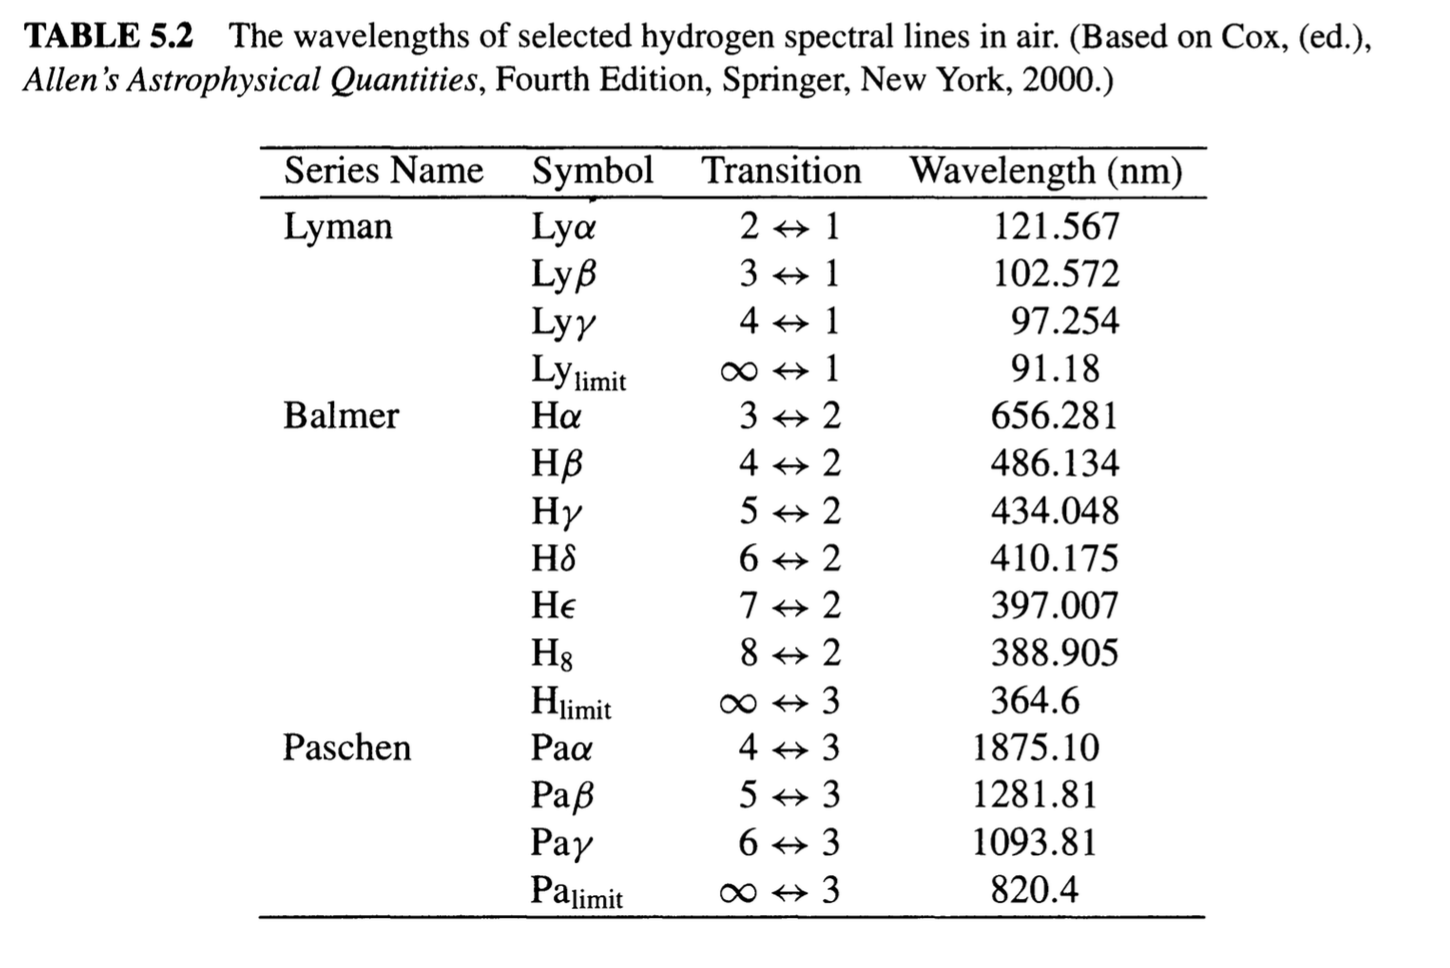
\includegraphics[width=5in]{CandOfigs/hydrogen_lines.png}
\end{figure}
\item Bohr model: angular momentum is quantized - $L = n\hbar$
\begin{equation}
{\bf F} = \frac{1}{4\pi\epsilon_0}\frac{q_1q_2}{r^2}\hat{\bf r}~~(\text{SI}) = \frac{q_1q_2}{r^2}\hat{\bf r}~~(\text{cgs})
\end{equation}
Coulomb force equals centripetal force:
\begin{equation}
\frac{q_1q_2}{r^2}\hat{\bf r} = -\mu \frac{v^2}{r}\hat{\bf r}
\end{equation}
\begin{equation}
\Longrightarrow K = \frac{1}{2}\mu v^2 = \frac{1}{2}\frac{e^2}{r}
\end{equation}
Potential energy is
\begin{equation}
U = -\frac{e^2}{r} = -2K
\end{equation}
So, 
\begin{equation}
E = K+U = K - 2K = -K = -\frac{e^2}{r}
\end{equation}
Requiring quantization of angular momentum:
\begin{equation}
L = \mu v r = n \hbar
\end{equation}
\begin{equation}
\Longrightarrow K = \frac{1}{2}\frac{e^2}{r} = \frac{1}{2}\mu v^2 = \frac{1}{2}\frac{(\mu v r)^2}{\mu r^2} = \frac{1}{2}\frac{(n\hbar)^2}{\mu r^2}
\end{equation}
\begin{equation}
\Longrightarrow r_n = \frac{\hbar^2}{\mu e^2}n^2 = a_0 n^2,
\end{equation}
$a_0 = 5.29\times 10^{-11}\text{ m}$.
\begin{equation}
\Longrightarrow E_n = -13.6\text{ eV}\frac{1}{n^2}
\end{equation}
\item de Broglie: Wave-partical duality of everything, not just light: $\nu = E/h$, $\lambda = h/p$

\item Heisenberg's uncertainty principle:
\begin{equation}
\Delta x \Delta p \ge \frac{1}{2}\hbar
\end{equation}
\begin{equation}
\Delta E \Delta t \ge \frac{1}{2} \hbar
\end{equation}

\item Schr\"odinger
\begin{equation}
L = \sqrt{l(l+1)}\hbar,~~~l = 0, 1, 2, \dots, n-1
\end{equation}
$z$-component of angular momentum vector, $L_z$ can only assume
\begin{equation}
L_z = m_l \hbar,~~~m_l = -l,-l+1, \dots, l-1, l
\end{equation}
\item Zeeman effect: splitting of spectral lines in weak magnetic field:
\begin{equation}
\nu = \nu_0~~~~~\text{ and }~~~~~\nu_0\pm\frac{eB}{4\pi\mu}
\end{equation}
\item Spin:
\begin{equation}
S = \sqrt{\frac{1}{2}\left(\frac{1}{2}+1\right)}\hbar = \frac{\sqrt{3}}{2}\hbar,
\end{equation}
$z$-component
\begin{equation}
S_z = m_s\hbar,~~~m_s = \pm\frac{1}{2}
\end{equation}
\item Pauli exclusion principle: no two electrons can share the same set of four quantum numbers
\item Dirac:
\begin{itemize}
\item Fermions: 
\begin{itemize}
\item electrons, protons, neutrons
\item spin of $(n+1)\hbar/2$, $n\in\mathbb{Z}$
\item obey Pauli exclusion principle
\end{itemize}
\item Bosons:
\begin{itemize}
\item ex. photons
\item spin of $n\hbar$, $n\in\mathbb{Z}$
\item do not obey the Pauli exclusion principle
\end{itemize}
\item predicted antiparticles
\begin{itemize}
\item identical, except for opposite electric charges and magnetic moments
\item Can be created from energy of gamma-ray photons, and can annihilate
\end{itemize}
\end{itemize}
\item Selection rules:
\begin{itemize}
\item $\Delta l = \pm 1$
\item $\Delta m_l = 0$ or $\pm 1$
\end{itemize}
\begin{itemize}
\item Allowed transitions: can happen spontaneously on timescales of 10$^{-8}$ s
\item Forbidden transitions: can occur, but require much longer times if they are to occur with any significant probability
\\ **Low gas densities are required for measurable intensities to be observed from forbidden transitions since collisions trigger transitions
\\ -- ISM or outer atmospheres of stars
\end{itemize}
\end{itemize}

\section{Telescopes}
\begin{itemize}
\item Snell's law:
\begin{equation}
n_{1,\lambda}\sin\theta_1 = n_{2,\theta}\sin\theta_2,
\end{equation}
$n_\lambda \equiv c/v_\lambda$
\item Focal point: point at which rays converge
\item Focal length, $f$: positive for a converging lens, negative for a diverging lens
\item Lensmaker's formula:
\begin{equation}
\frac{1}{f_\lambda} = (n_\lambda - 1)\left(\frac{1}{R_1} + \frac{1}{R_2}\right),
\end{equation}
where $R_1$ and $R_2$ are the radii of curvature of each surface. Positive if convex, negative if concave.
\item ***For mirrors, $f$ is wavelength independent since 
\item ***For a spheroidal mirror, $f = R/2$
\item Focal plane: plane passing through the focal point and oriented perpendicular to the optical axis
\item Two point sources separated by angle $\theta$ will be separated by
\begin{equation}
y = f\tan \theta \approx f\theta
\end{equation}
on the focal plane.
\begin{figure}[h!]
\centering
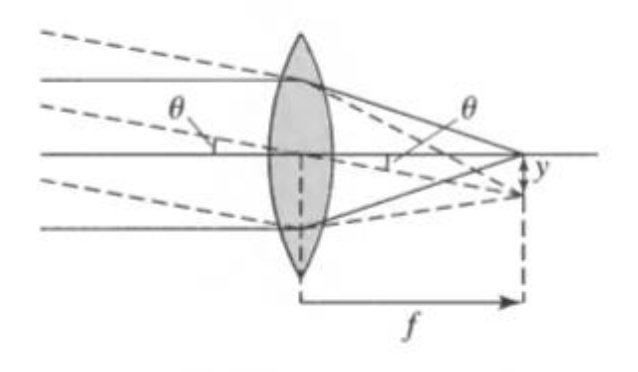
\includegraphics[width=3in]{CandOfigs/pointsources_focalplane.png}
\end{figure}
\item Plate scale:
\begin{equation}
\frac{d\theta}{dy} = \frac{1}{f}
\end{equation}
\item Rayleigh Criterion:
\begin{equation}
\theta_\text{min} = 1.22\frac{\lambda}{D}
\end{equation}
\begin{itemize}
\item Single slit diffraction:\\
Slit of width $D$, consider rays from edge of slit and center of slit: Leads to destructive interference when
\begin{equation}
\frac{D}{2}\sin\theta = \frac{1}{2}\lambda
\end{equation}
Can divide into four segments to get destructive interference when
\begin{equation}
\frac{D}{4}\sin\theta = \frac{1}{2}\lambda
\end{equation}
Put together, destructive interference at
\begin{equation}
\sin\theta = m\frac{\lambda}{D},~~~m=1,2,3,\dots
\end{equation}
\item Airy disk: In 2D, $m$ describes maxima and minima and is no longer integer:
\begin{figure}[h!]
\centering
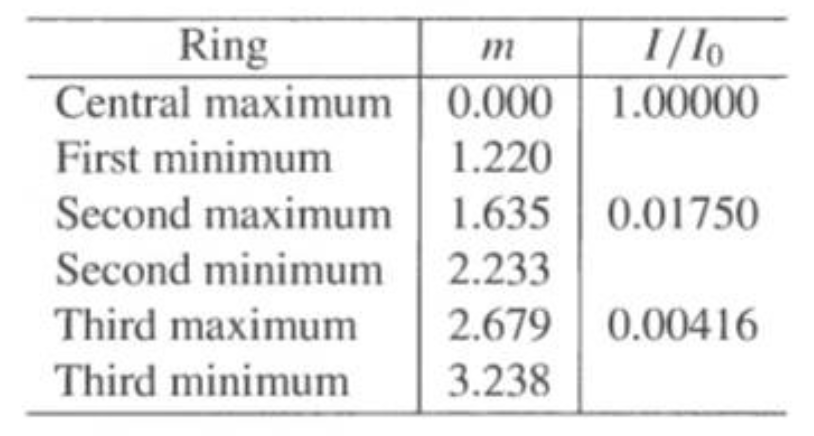
\includegraphics[width=3in]{CandOfigs/airyrings.png}
\end{figure}
\end{itemize}

\item Seeing: resolution suffers from atmospheric turbulence
\begin{itemize}
\item Mauna Kea: $0.5^{\prime\prime}$ to $0.6^{\prime\prime}$ 50\% of the time, and $0.25^{\prime\prime}$ on the best nights
\item Other sites with good seeing: Kitt Peak, Tenerife and La Palma of the Canary Islands, several sites in the Chilean Andes Mountains (Cerro Tololo Inter-American Observatory, the Cerro La Silla and Cerro Paranal sites of the ESO, and Cerro Pach\'on, location of Gemini South)
\end{itemize}
\item Aberrations
\begin{itemize}
\item Chromatic aberration: focal length is wavelength dependent. Can use correcting lenses to diminish this effect
\item Spherical aberration: Not all areas of surfaces will focus parallel rays to a single point. Can use paraboloid instead, but more expensive. ***This was the problem with Hubble
\item Coma: elongated images of point sources that lie off the optical axis because of focal length dependence on $\theta$
\item Astigmatism: different parts of a lens or mirror converge an image at slightly different locations on the focal plane. Can design a lens to correct for astigmatism, but then....
\item curvature of field: focuses images on a curve rather than on a plane.
\item Distortion of field: when the plate scale depends on the distance from the optical axis
\end{itemize}

\item Brightness of Image
\begin{figure}[h!]
\centering
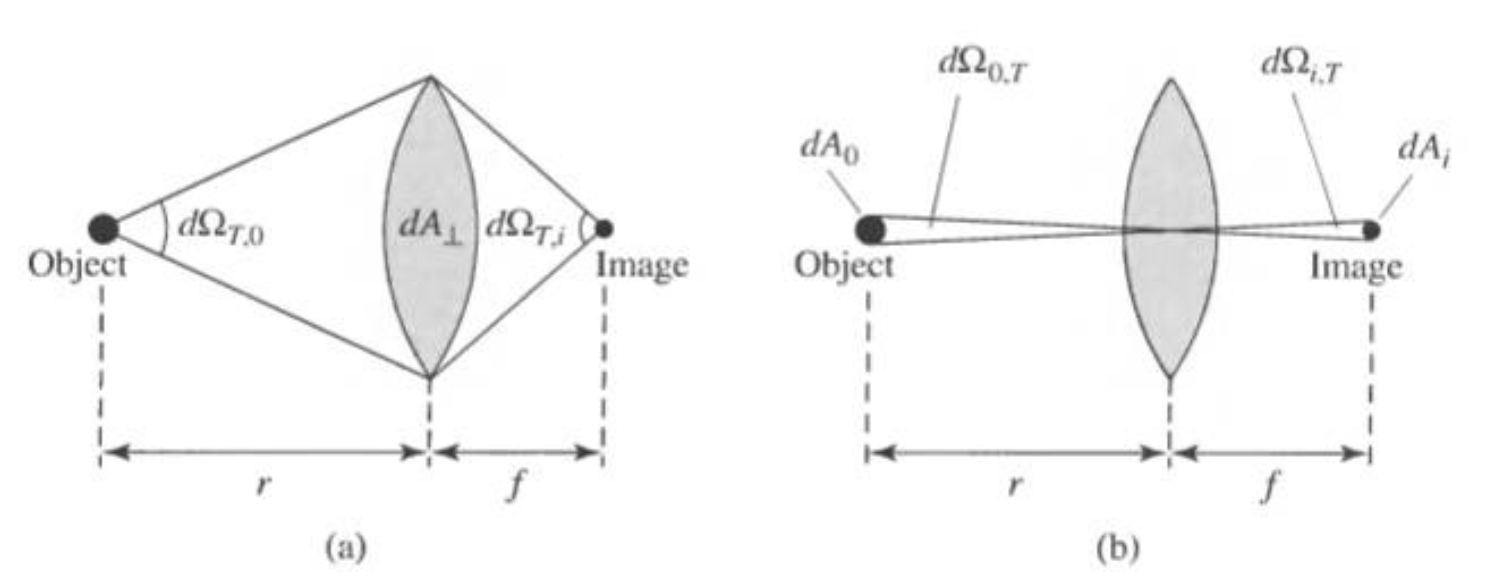
\includegraphics[width=5in]{CandOfigs/objectandimagesolidangles.png}
\end{figure}
\begin{itemize}
\item If surface area $dA_O$ of object at distance $r$ has surface intensity $I_O$, then energy per second per unit wavelength radiated into telescope with solid angle $d\Omega_{T,O}$ is
\begin{equation}
I_O d\Omega_{T,O} dA_O = I_O\left(\frac{A_T}{r^2}\right)dA_O,
\end{equation}
where $A_T$ is the area of telescope's aperture. Also, all the photons emitted going into solid angle $\Omega_{T,O}$ will strike an area $dA_{i}$ on the focal plane, 
\begin{equation}
I_O d\Omega_{T,O} dA_O = I_i d\Omega_{T,i} dA_{i},
\end{equation}
where $I_i$ is the image intensity and $d\Omega_{T,i}$ is the solid angle defined by the telescope's aperture as seen from the image.
\begin{equation}
\Longrightarrow  I_O\left(\frac{A_T}{r^2}\right)dA_O = I_i\left(\frac{A_T}{f^2}\right)dA_i
\end{equation}
\begin{equation}
\Longrightarrow I_i = I_O\left(\frac{dA_O/r^2}{dA_i/f^2}\right)
\end{equation}
If we look {\textit from} the lens, $d\Omega_{O,T} = d\Omega_{i,T}$, so 
\begin{equation}
\frac{dA_O}{r^2} = \frac{d A_i}{f^2}
\end{equation}
\begin{equation}
\Longrightarrow I_i = I_O
\end{equation}
This shows that the image intensity is identical to the object intensity, independent of the area of the aperture.
\end{itemize}
\item Illumination $J$: the amount of light energy per second focused onto a unit area of the resolved image, so 
\begin{equation}
J \propto D^2/f^2
\end{equation}
\item Focal ratio:
\begin{equation}
F \equiv \frac{f}{D} \Longrightarrow J \propto	\frac{1}{F^2}
\end{equation}
--Keck: $f = 17.5\text{ m}$, $D = 10\text{ m}$ $\Longrightarrow F = 1.75$

\item Optical telescopes:
\begin{itemize}
\item Refracting:
\begin{itemize}
\item Objective (primary) lens with $f_\text{obj}$ and eyepiece which magnifies:
\begin{equation}
m = \frac{f_\text{obj}}{f_\text{eye}}
\end{equation}
\item Limited in size by deformation due to gravity -- need to support primary. Deformation will change according to orientation
\item Hard to construct lens sufficiently free of defects -- large volume to perfect
\item Defects must be kept less than $\sim\lambda/20$
\item Slow thermal response and a lot of thermal expansion
\item Lots of torque with large detectors
\end{itemize}
\item Reflecting:
\begin{itemize}
\item Only one surface to perfect
\item Reduce weight with honeycomb  structure
\item Can support from back of mirror and so can use pressure pads to correct for distortions
\item Prime focus is in the path of incoming light
\item Schmidt telescopes: Wide angle field of view $\sim$several degrees
\begin{figure}[h!]
\centering
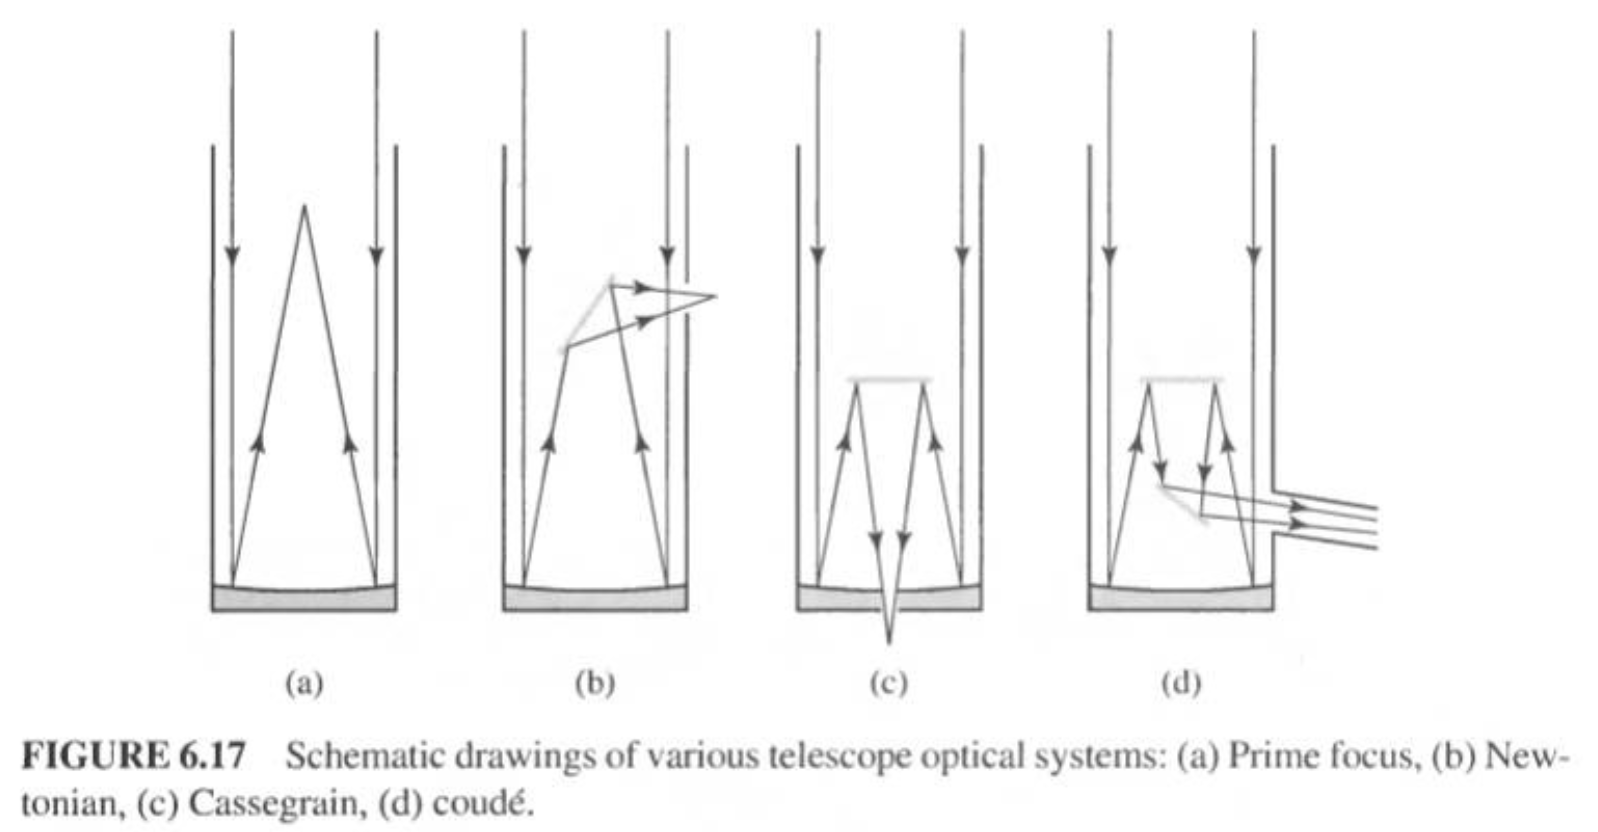
\includegraphics[width=6in]{CandOfigs/telescopetypes.png}
\end{figure}
\end{itemize}
\item Mounts
\begin{itemize}
\item Equatorial: 
\begin{itemize}
\item Polar axis, so simply need to rotate to adjust ra
\item Expensive and difficult to build for large telescopes
\end{itemize}
\item Altitude-azimuth:
\begin{itemize}
\item motion parallel and perpendicular to horizon
\item Tracking of objects requires continuous calculation
\end{itemize}
\end{itemize}
\item AO:
\begin{itemize}
\item deformable mirror with piezoelectric crystals on back
\item Micrometer-size adjustments, several hundred times per second
\item Use guide star to determine adjustments
\item If no guide star, use laser, exciting sodium atoms $\sim90$ km altitude
\item Good for near-infrared because of longer wavelengths
\end{itemize}
\item Space-based:
\begin{itemize}
\item Hubble:
\begin{itemize}
\item 2.4-m, $f$/24
\item down to 30th magnitude
\item 120 nm to 1 $\mu$m -- UV to infrared
\item Ritchey-Chr\'etien -- (hyperbolic primary, Cassegrain)
\end{itemize}
\item JWST:
\begin{itemize}
\item 6-m
\item 600 nm to 28 $\mu$m
\item Located at L2 (away from Sun)
\end{itemize}
\end{itemize}
\end{itemize}
\item Radio telescopes
\begin{itemize}
\item 
\end{itemize}
\end{itemize}


\section*{Chapter 7}

\section*{Chapter 8}

\section*{Chapter 9}

\section*{Chapter 10}

\end{document}